\documentclass[12pt,a4paper]{article}

% --- Pakete ---
\usepackage[utf8]{inputenc}
\usepackage[T1]{fontenc}
\usepackage[ngerman]{babel}
\usepackage{graphicx}
\usepackage{csquotes}
\usepackage{amsmath}
\usepackage{geometry}
\usepackage{hyperref}
\usepackage{biblatex}
\addbibresource{literatur.bib}

% --- Seitenränder ---
\geometry{margin=2.5cm}

% --- Metadaten ---
\title{Automatische Levelgenerierung mit Unity}
\author{Adrian Weiner \\ Matrikelnummer: 10014650}
\date{\today}

% --- Dokumentstart ---
\begin{document}

\maketitle

\tableofcontents
\newpage

% --- Kapitel (können in Dateien ausgelagert sein) ---
\section{Einleitung}

Diese Arbeit beschäftigt sich mit der automatischen Generierung von Levelstrukturen
für ein 3D-Jump’n’Run-Spiel in der Unity Engine.

Ziel ist die Entwicklung eines Systems, das mit jedem Level den Schwierigkeitsgrad
dynamisch anpasst – basierend auf zufälliger Verteilung, Regeln und Spielbarkeit.


\section{Abbildungen}
Beispielabbildung:

\begin{figure}[h]
    \centering
    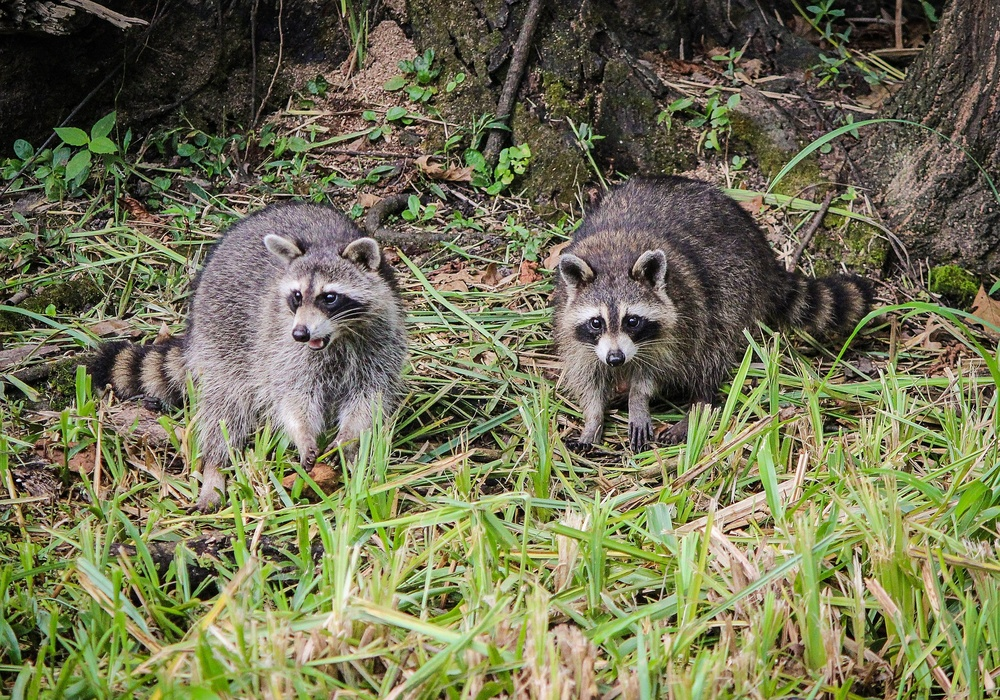
\includegraphics[width=0.8\textwidth]{bilder/beispielbild.png}
    \caption{Levelstruktur im Prototyp}
\end{figure}

\section{Fazit}
Hier steht dein Fazit.

% --- Literaturverzeichnis ---
\printbibliography

\end{document}
